% Practice Test 02 — Texas Edition
% Questions: 30 (22 MC + 8 SA)
% Generated by scripts/generate_practice_tests.py

\begin{practiceQuestion}{1-3-q30}{gsa}
\begin{questionText}
The table shows a proportional relationship between minutes and laps completed. Find $k$ and determine how many laps are completed in $15$ minutes.

\begin{center}
\begin{tabular}{|c|c|}
\hline
\textbf{Minutes ($x$)} & \textbf{Laps ($y$)} \\ \hline
$4$ & $3$ \\ \hline
$8$ & $6$ \\ \hline
$12$ & $9$ \\ \hline
$15$ & $?$ \\ \hline
\end{tabular}
\end{center}
\end{questionText}
\correctAnswer{$k = 0.75$; $11.25$ laps in $15$ minutes}
\explanation{$k = \frac{3}{4} = 0.75$. For $15$ minutes: $y = 0.75 \times 15 = 11.25$ laps.}
\end{practiceQuestion}

\begin{practiceQuestion}{1-6-q07}{mc}
\begin{questionText}
On a map, $3$ cm represents $24$ km. How far apart are two towns that are $8$ cm apart on the map?
\end{questionText}
\choiceA{$48$ km}
\choiceB{$56$ km}
\choiceC{$64$ km}
\choiceD{$72$ km}
\correctAnswer{C}
\explanation{$\frac{3}{24} = \frac{8}{d}$. Cross-multiply: $3d = 192$, so $d = 64$ km.}
\end{practiceQuestion}

\begin{practiceQuestion}{2-1-q25}{sa}
\begin{questionText}
A parking lot has spaces for $350$ cars. Currently $280$ spaces are filled. What percent of the lot is full?
\end{questionText}
\correctAnswer{$80\%$}
\explanation{Divide: $280 \div 350 = 0.80 = 80\%$.}
\end{practiceQuestion}

\begin{practiceQuestion}{2-3-q13}{mc}
\begin{questionText}
A $\$250$ tablet is on sale for $20\%$ off. A student says the sale price is $\$200$. Another student says it is $\$230$. Who is correct?


\numberLine[5]{200}{255}
\end{questionText}
\choiceA{The first student ($\$200$)}
\choiceB{The second student ($\$230$)}
\choiceC{Neither student}
\choiceD{Both students}
\correctAnswer{A}
\explanation{$20\%$ off: $250 \times 0.80 = \$200$. The first student is correct.}
\end{practiceQuestion}

\begin{practiceQuestion}{2-6-q06}{mc}
\begin{questionText}
Which gives more interest: $\$600$ at $4\%$ for $3$ years, or $\$600$ at $3\%$ for $4$ years?
\end{questionText}
\choiceA{$4\%$ for $3$ years}
\choiceB{$3\%$ for $4$ years}
\choiceC{They give the same interest}
\choiceD{Cannot be determined}
\correctAnswer{C}
\explanation{Option 1: $600 \times 0.04 \times 3 = \$72$. Option 2: $600 \times 0.03 \times 4 = \$72$. They are equal.}
\end{practiceQuestion}

\begin{practiceQuestion}{2-8-q10}{mc}
\begin{questionText}
Compared to a bank, a credit union typically offers:
\end{questionText}
\choiceA{Higher fees and higher interest rates on loans}
\choiceB{No savings accounts}
\choiceC{Lower fees and is owned by its members}
\choiceD{Government-backed stock investments}
\correctAnswer{C}
\explanation{Credit unions are member-owned and often charge lower fees than banks.}
\end{practiceQuestion}

\begin{practiceQuestion}{2-9-q30}{gsa}
\begin{questionText}
The bar graph shows two people's monthly budgets. Who saves more money, and by how much?

\begin{center}
\begin{tikzpicture}[scale=0.55]
  \draw[thick,->] (0,0) -- (0,7) node[above] {\$};
  \draw[thick,->] (0,0) -- (12,0);
  \foreach \y/\label in {0/0, 1/200, 2/400, 3/600, 4/800, 5/1000, 6/1200} {
    \draw (-0.1,\y) -- (0.1,\y);
    \node[left] at (-0.15,\y) {\footnotesize \$\label};
  }
  % Alex
  \fill[funBlue!50] (0.5,0) rectangle (1.8,5);
  \node[below] at (1.15,0) {\footnotesize Income};
  \node[above] at (1.15,5) {\footnotesize \$1000};
  \fill[funRed!50] (2.2,0) rectangle (3.5,4);
  \node[below] at (2.85,0) {\footnotesize Expenses};
  \node[above] at (2.85,4) {\footnotesize \$800};
  \node[below] at (2,-0.8) {\footnotesize Alex};

  % Beth
  \fill[funBlue!50] (6,0) rectangle (7.3,6);
  \node[below] at (6.65,0) {\footnotesize Income};
  \node[above] at (6.65,6) {\footnotesize \$1200};
  \fill[funRed!50] (7.7,0) rectangle (9,5.25);
  \node[below] at (8.35,0) {\footnotesize Expenses};
  \node[above] at (8.35,5.25) {\footnotesize \$1050};
  \node[below] at (7.5,-0.8) {\footnotesize Beth};
\end{tikzpicture}
\end{center}
\end{questionText}
\correctAnswer{Alex by $\$50$}
\explanation{Alex saves: $1{,}000 - 800 = \$200$. Beth saves: $1{,}200 - 1{,}050 = \$150$. Alex saves $200 - 150 = \$50$ more.}
\end{practiceQuestion}

\begin{practiceQuestion}{2-10-q01}{mc}
\begin{questionText}
What is the main difference between simple and compound interest?
\end{questionText}
\choiceA{Simple interest uses a higher rate}
\choiceB{Compound interest is calculated on the principal plus previously earned interest}
\choiceC{Simple interest compounds monthly}
\choiceD{Compound interest only applies to loans}
\correctAnswer{B}
\explanation{Compound interest is calculated on the principal plus any interest already earned, so your interest earns interest.}
\end{practiceQuestion}

\begin{practiceQuestion}{4-1-q23}{sa}
\begin{questionText}
A cell phone plan charges $c$ cents per minute. Write an expression for the cost of a $15$-minute call in dollars.
\end{questionText}
\correctAnswer{$\frac{15c}{100}$ or $0.15c$}
\explanation{$15$ minutes at $c$ cents each is $15c$ cents. To convert to dollars, divide by $100$: $\frac{15c}{100} = 0.15c$.}
\end{practiceQuestion}

\begin{practiceQuestion}{4-2-q15}{mc}
\begin{questionText}
Simplify $10 - 3x + 5x - 4$.
\end{questionText}
\choiceA{$8x + 6$}
\choiceB{$-8x + 6$}
\choiceC{$2x + 6$}
\choiceD{$2x - 6$}
\correctAnswer{C}
\explanation{Combine variable terms: $-3x + 5x = 2x$. Combine constants: $10 - 4 = 6$. Result: $2x + 6$.}
\end{practiceQuestion}

\begin{practiceQuestion}{5-3-q21}{sa}
\begin{questionText}
Solve $5(2x - 3) = 35$.
\end{questionText}
\correctAnswer{$x = 5$}
\explanation{Divide by $5$: $2x - 3 = 7$. Add $3$: $2x = 10$. Divide by $2$: $x = 5$. Check: $5(2(5) - 3) = 5(7) = 35$ \checkmark.}
\end{practiceQuestion}

\begin{practiceQuestion}{5-4-q05}{mc}
\begin{questionText}
Solve $\dfrac{2x}{5} - 1 = 3$.
\end{questionText}
\choiceA{$x = 5$}
\choiceB{$x = 10$}
\choiceC{$x = 4$}
\choiceD{$x = 20$}
\correctAnswer{B}
\explanation{Add $1$: $\frac{2x}{5} = 4$. Multiply by $5$: $2x = 20$. Divide by $2$: $x = 10$. Check: $\frac{2(10)}{5} - 1 = 4 - 1 = 3$ \checkmark.}
\end{practiceQuestion}

\begin{practiceQuestion}{5-5-q09}{mc}
\begin{questionText}
A student solved $-2x + 8 > 14$ and wrote $x > -3$. What error did the student make?
\end{questionText}
\choiceA{Forgot to subtract $8$}
\choiceB{Divided by $2$ instead of $-2$}
\choiceC{Forgot to flip the inequality sign}
\choiceD{Added $8$ instead of subtracting}
\correctAnswer{C}
\explanation{Correct steps: subtract $8$ → $-2x > 6$. Divide by $-2$ and flip: $x < -3$. The student forgot to flip.}
\end{practiceQuestion}

\begin{practiceQuestion}{5-6-q12}{mc}
\begin{questionText}
Solve $2x - 1 < 7$ and describe the graph.
\end{questionText}
\choiceA{Open circle at $4$, shade left}
\choiceB{Closed circle at $4$, shade left}
\choiceC{Open circle at $3$, shade left}
\choiceD{Open circle at $4$, shade right}
\correctAnswer{A}
\explanation{Add $1$: $2x < 8$. Divide by $2$: $x < 4$. Open circle at $4$, shade left.}
\end{practiceQuestion}

\begin{practiceQuestion}{6-2-q04}{mc}
\begin{questionText}
A drawing uses $1$ cm $= 3$ m. It is redrawn at $1$ cm $= 9$ m. A room that is $12$ cm on the original becomes how long?
\end{questionText}
\choiceA{$4$ cm}
\choiceB{$12$ cm}
\choiceC{$36$ cm}
\choiceD{$108$ cm}
\correctAnswer{A}
\explanation{Scale ratio: $\frac{3}{9} = \frac{1}{3}$. New length: $12 \times \frac{1}{3} = 4$ cm.}
\end{practiceQuestion}

\begin{practiceQuestion}{6-3-q16}{mc}
\begin{questionText}
A parallelogram has side lengths $5$ cm and $8$ cm. How many different parallelograms can be drawn?
\end{questionText}
\choiceA{None}
\choiceB{Exactly one}
\choiceC{Exactly two}
\choiceD{More than one}
\correctAnswer{D}
\explanation{Two side lengths of a parallelogram do not fix the angles. The shape can be a rectangle, a rhomboid, or anything in between. Many different parallelograms are possible.}
\end{practiceQuestion}

\begin{practiceQuestion}{6-4-q26}{gmc}
\begin{questionText}
The diagram shows a triangle with the given angle measures. Is this a valid triangle?

\begin{center}
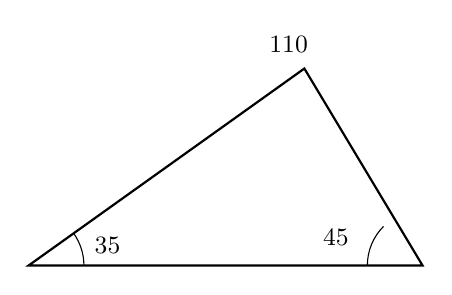
\begin{tikzpicture}[scale=1]
  \draw[thick] (0,0) -- (5,0) -- (3.5,2.5) -- cycle;
  \draw (0.7,0) arc[start angle=0,end angle=35,radius=0.7];
  \node at (1.0,0.25) {\small $35°$};
  \draw (4.3,0) arc[start angle=180,end angle=135,radius=0.7];
  \node at (3.9,0.35) {\small $45°$};
  \node at (3.3,2.8) {\small $110°$};
\end{tikzpicture}
\end{center}
\end{questionText}
\choiceA{Yes, because $35 + 45 + 110 = 190$}
\choiceB{Yes, because all angles are positive}
\choiceC{No, because the angles sum to $190°$ instead of $180°$}
\choiceD{No, because one angle is greater than $90°$}
\correctAnswer{C}
\explanation{$35 + 45 + 110 = 190 \neq 180$. Triangle angles must sum to exactly $180°$, so this triangle is not valid.}
\end{practiceQuestion}

\begin{practiceQuestion}{6-5-q07}{mc}
\begin{questionText}
A triangular prism is sliced with a cut parallel to its triangular base. What is the cross-section?
\end{questionText}
\choiceA{A rectangle}
\choiceB{A triangle congruent to the base}
\choiceC{A smaller triangle}
\choiceD{A trapezoid}
\correctAnswer{B}
\explanation{A cut parallel to the base of a prism always produces a shape congruent (same size and shape) to the base. For a triangular prism, this is a triangle identical to the base.}
\end{practiceQuestion}

\begin{practiceQuestion}{6-8-q28}{gmc}
\begin{questionText}
The diagram below shows a person and a flagpole casting shadows at the same time. What is the height of the flagpole?

\begin{center}
\begin{tikzpicture}[scale=0.35]
  % Person
  \draw[thick] (0,0) -- (0,4);
  \draw[thick] (0,0) -- (3,0);
  \draw[dashed] (0,4) -- (3,0);
  \node[left] at (0,2) {$4$ ft};
  \node[below] at (1.5,0) {$3$ ft};
  % Flagpole
  \draw[thick] (6,0) -- (6,12);
  \draw[thick] (6,0) -- (15,0);
  \draw[dashed] (6,12) -- (15,0);
  \node[left] at (6,6) {$h$};
  \node[below] at (10.5,0) {$9$ ft};
  % Ground
  \draw[thick] (-1,0) -- (16,0);
\end{tikzpicture}
\end{center}
\end{questionText}
\choiceA{$6$ ft}
\choiceB{$12$ ft}
\choiceC{$16$ ft}
\choiceD{$36$ ft}
\correctAnswer{B}
\explanation{$\frac{4}{3} = \frac{h}{9}$. Cross-multiply: $3h = 36$. Divide: $h = 12$ ft.}
\end{practiceQuestion}

\begin{practiceQuestion}{7-4-q29}{gsa}
\begin{questionText}
Find the area of the shaded L-shaped figure shown below. Each square on the grid is $1$ ft by $1$ ft.

\begin{center}
\begin{tikzpicture}[scale=0.5]
  \draw[step=1,gray!30,thin] (0,0) grid (8,8);
  \fill[funBlue!20] (1,1) -- (7,1) -- (7,5) -- (4,5) -- (4,7) -- (1,7) -- cycle;
  \draw[thick,funBlue] (1,1) -- (7,1) -- (7,5) -- (4,5) -- (4,7) -- (1,7) -- cycle;
  \node[below] at (4,0.8) {$6$};
  \node[right] at (7.2,3) {$4$};
  \node[above] at (2.5,7.2) {$3$};
  \node[left] at (0.8,4) {$6$};
\end{tikzpicture}
\end{center}
\end{questionText}
\correctAnswer{$30$ ft$^2$}
\explanation{Bottom rectangle: $6 \times 4 = 24$ ft$^2$. Top-left rectangle: $3 \times 2 = 6$ ft$^2$. Total: $24 + 6 = 30$ ft$^2$.}
\end{practiceQuestion}

\begin{practiceQuestion}{7-5-q12}{mc}
\begin{questionText}
A storage box is in the shape of a cube with side $12$ inches. What is its surface area?
\end{questionText}
\choiceA{$144$ in$^2$}
\choiceB{$432$ in$^2$}
\choiceC{$864$ in$^2$}
\choiceD{$1728$ in$^2$}
\correctAnswer{C}
\explanation{$SA = 6s^2 = 6 \times 144 = 864$ in$^2$.}
\end{practiceQuestion}

\begin{practiceQuestion}{7-6-q28}{gmc}
\begin{questionText}
A triangular prism is shown below. What is its volume?

\begin{center}
\begin{tikzpicture}[scale=0.35]
  % Front triangle
  \fill[funBlue!10] (0,0) -- (8,0) -- (4,5) -- cycle;
  \draw[thick,funBlue] (0,0) -- (8,0) -- (4,5) -- cycle;
  % Back triangle
  \fill[funBlue!20] (3,2) -- (11,2) -- (7,7) -- cycle;
  \draw[thick,funBlue] (3,2) -- (11,2) -- (7,7) -- cycle;
  % Connecting edges
  \draw[thick,funBlue] (0,0) -- (3,2);
  \draw[thick,funBlue] (8,0) -- (11,2);
  \draw[thick,funBlue] (4,5) -- (7,7);
  % Labels
  \draw[thick,funRed,<->] (0,-0.8) -- (8,-0.8);
  \node[below,funRed] at (4,-0.8) {$8$ m};
  \draw[dashed,gray] (4,0) -- (4,5);
  \node[left,funRed] at (3.8,2.5) {$5$ m};
  \node[right,funRed] at (11.2,4.5) {$12$ m};
\end{tikzpicture}
\end{center}
\end{questionText}
\choiceA{$120$ m$^3$}
\choiceB{$240$ m$^3$}
\choiceC{$480$ m$^3$}
\choiceD{$96$ m$^3$}
\correctAnswer{B}
\explanation{$B = \frac{1}{2} \times 8 \times 5 = 20$ m$^2$. $V = 20 \times 12 = 240$ m$^3$.}
\end{practiceQuestion}

\begin{practiceQuestion}{8-1-q13}{mc}
\begin{questionText}
A manager surveys every $20$th customer who enters a store. This is an example of:
\end{questionText}
\choiceA{A voluntary sample}
\choiceB{A convenience sample}
\choiceC{A systematic sample}
\choiceD{A biased sample}
\correctAnswer{C}
\explanation{Selecting every $n$th member is called systematic sampling.}
\end{practiceQuestion}

\begin{practiceQuestion}{8-2-q10}{mc}
\begin{questionText}
A random sample of $100$ households found an average of $2.4$ pets per household. Predict the total number of pets in a town of $5{,}000$ households.
\end{questionText}
\choiceA{$2{,}400$}
\choiceB{$5{,}000$}
\choiceC{$12{,}000$}
\choiceD{$24{,}000$}
\correctAnswer{C}
\explanation{$5{,}000 \times 2.4 = 12{,}000$ pets.}
\end{practiceQuestion}

\begin{practiceQuestion}{8-4-q08}{mc}
\begin{questionText}
Class P: mean $70$, median $72$, range $15$, MAD $4$.
Class Q: mean $68$, median $67$, range $35$, MAD $9$.
Which class has more consistent scores?
\end{questionText}
\choiceA{Class P}
\choiceB{Class Q}
\choiceC{Both are equally consistent}
\choiceD{Cannot be determined}
\correctAnswer{A}
\explanation{Class P has smaller range ($15$ vs.\ $35$) and smaller MAD ($4$ vs.\ $9$), meaning its scores are more tightly clustered.}
\end{practiceQuestion}

\begin{practiceQuestion}{8-5-q06}{mc}
\begin{questionText}
Using the stem-and-leaf plot in the previous question, what is the smallest data value?
\end{questionText}
\choiceA{$42$}
\choiceB{$4$}
\choiceC{$2$}
\choiceD{$45$}
\correctAnswer{A}
\explanation{The first stem is $4$ and the first leaf is $2$, so the smallest value is $42$.}
\end{practiceQuestion}

\begin{practiceQuestion}{8-6-q29}{gsa}
\begin{questionText}
The circle graph shows a family's monthly budget of $\$4{,}000$.

\begin{center}
\begin{tikzpicture}[scale=1.3]
  % Housing 35%, Food 20%, Transport 15%, Savings 10%, Other 20%
  % Angles: 126, 72, 54, 36, 72
  \fill[funBlue!50] (0,0) -- (90:1.5) arc (90:90-126:1.5) -- cycle;
  \fill[funGreen!50] (0,0) -- (90-126:1.5) arc (90-126:90-126-72:1.5) -- cycle;
  \fill[funOrange!50] (0,0) -- (90-126-72:1.5) arc (90-126-72:90-126-72-54:1.5) -- cycle;
  \fill[funRed!40] (0,0) -- (90-126-72-54:1.5) arc (90-126-72-54:90-126-72-54-36:1.5) -- cycle;
  \fill[gray!30] (0,0) -- (90-126-72-54-36:1.5) arc (90-126-72-54-36:90:1.5) -- cycle;
  \draw (0,0) circle (1.5);
  \node[font=\small\bfseries] at (27:1.05) {Housing};
  \node[font=\tiny] at (27:0.65) {$35\%$};
  \node[font=\small\bfseries] at (-62:1.05) {Food};
  \node[font=\tiny] at (-62:0.65) {$20\%$};
  \node[font=\small\bfseries] at (-125:1.05) {Transport};
  \node[font=\tiny] at (-125:0.65) {$15\%$};
  \node[font=\small\bfseries] at (-160:1.05) {Savings};
  \node[font=\tiny] at (-160:0.65) {$10\%$};
  \node[font=\small\bfseries] at (145:1.05) {Other};
  \node[font=\tiny] at (145:0.65) {$20\%$};
\end{tikzpicture}
\end{center}

How much money is spent on food? How much is saved?
\end{questionText}
\correctAnswer{Food: $\$800$; Savings: $\$400$}
\explanation{Food: $20\%$ of $\$4{,}000 = \$800$. Savings: $10\%$ of $\$4{,}000 = \$400$.}
\end{practiceQuestion}

\begin{practiceQuestion}{9-4-q13}{mc}
\begin{questionText}
A probability model has outcomes A, B, and C with $P(A) = 0.5$ and $P(B) = 0.3$. What is $P(C)$?
\end{questionText}
\choiceA{$0.8$}
\choiceB{$0.3$}
\choiceC{$0.2$}
\choiceD{$0.1$}
\correctAnswer{C}
\explanation{All probabilities must sum to $1$. $P(C) = 1 - 0.5 - 0.3 = 0.2$.}
\end{practiceQuestion}

\begin{practiceQuestion}{9-6-q09}{mc}
\begin{questionText}
A bag has $3$ red and $2$ blue marbles. You draw one marble, replace it, and draw again. What is the probability that both are red?
\end{questionText}
\choiceA{$\frac{6}{25}$}
\choiceB{$\frac{9}{25}$}
\choiceC{$\frac{3}{10}$}
\choiceD{$\frac{6}{20}$}
\correctAnswer{B}
\explanation{With replacement: $P = \frac{3}{5} \times \frac{3}{5} = \frac{9}{25}$.}
\end{practiceQuestion}

\begin{practiceQuestion}{9-7-q22}{sa}
\begin{questionText}
A simulation of $50$ coin flips produces $22$ heads. Predict how many heads you would expect in $200$ flips based on this simulation.
\end{questionText}
\correctAnswer{$88$}
\explanation{Experimental $P(\text{heads}) = \frac{22}{50} = 0.44$. In $200$ flips: $200 \times 0.44 = 88$.}
\end{practiceQuestion}
